\documentclass{beamer}

\usepackage{import}
\usepackage{xifthen}
\usepackage{pdfpages}
\usepackage{transparent}
\usepackage{hyperref}
% \graphicspath{{../03_Reporte/img/}}

\mode<presentation>
{
  \usetheme{Berlin}
  \setbeamercovered{transparent}
    \setbeamertemplate{caption}[numbered]
  \setbeamertemplate{footline}[frame number]
}


\usepackage[spanish,mexico]{babel}
% \usepackage[utf8]{inputenc}
\usepackage{times}
\usepackage[T1]{fontenc}

\title{Plataforma Gough-Cappel}

\subtitle
{Comparación de gasto energético de estrategias de control}

\author[]{E. Benavides \and I. Ayala \and N. González}


\institute[]
{
  Centro de Investigación y de Estudios Acanzados del IPN\\
  Robótica y Manufactura Avanzada
  }

\date[]{RyMA 2019}

\subject{Robotics}



% Delete this, if you do not want the table of contents to pop up at
% the beginning of each subsection:
\AtBeginSubsection[]
{
  \begin{frame}<beamer>{Outline}
    \tableofcontents[currentsection,currentsubsection]
  \end{frame}
}


% If you wish to uncover everything in a step-wise fashion, uncomment
% the following command: 

%\beamerdefaultoverlayspecification{<+->}



\begin{document}

\begin{frame}
  \titlepage
\end{frame}

\begin{frame}{Contenido}
  \tableofcontents
\end{frame}



\section{Introducción}

\subsection{Nomenclatura}
\begin{frame}{Definiciones}
\begin{itemize}
    \item 
    \item 
    \item 
    \item 
    \item 
\end{itemize} 
\end{frame}

\section{Gasto Energético}
\subsection{Punto fijo}

\begin{frame}
 \begin{figure}
  \centering
  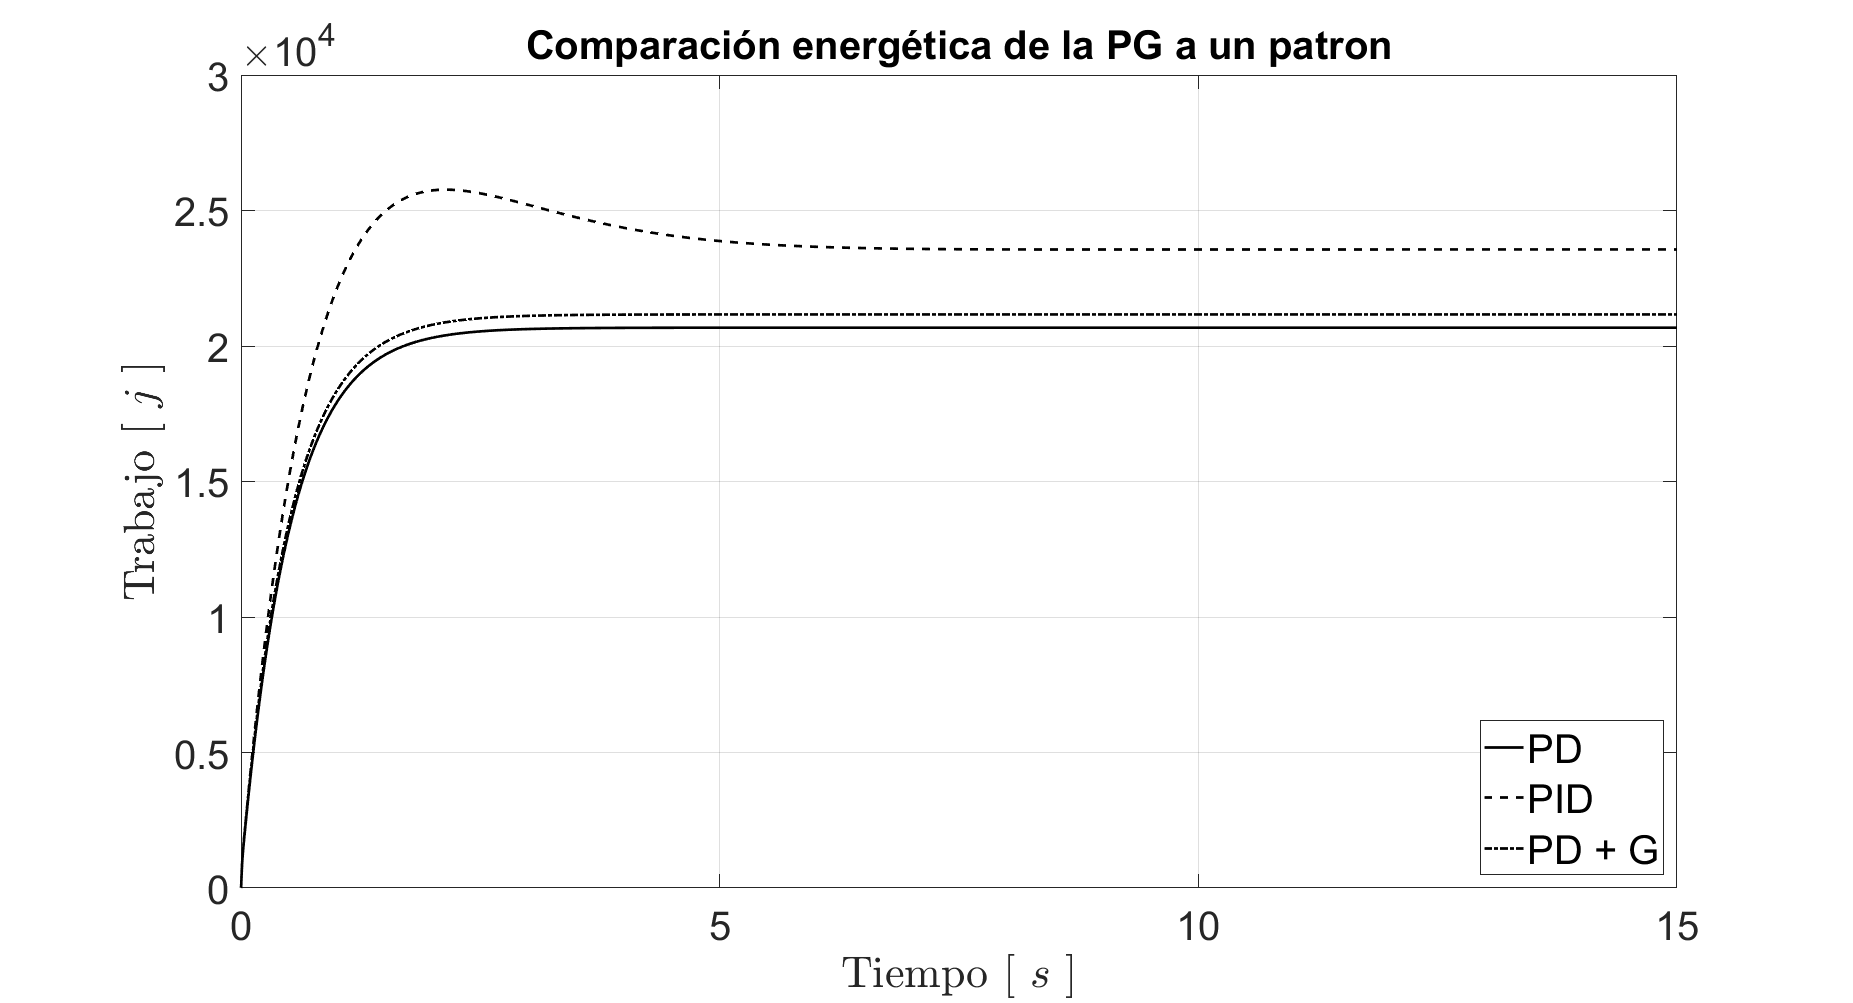
\includegraphics[width=\textwidth]{../03_Reporte/img/energiamov.png}
 \end{figure}

\end{frame}


\subsection{Trayectoria}
\begin{frame}
 \begin{figure}
  \centering
  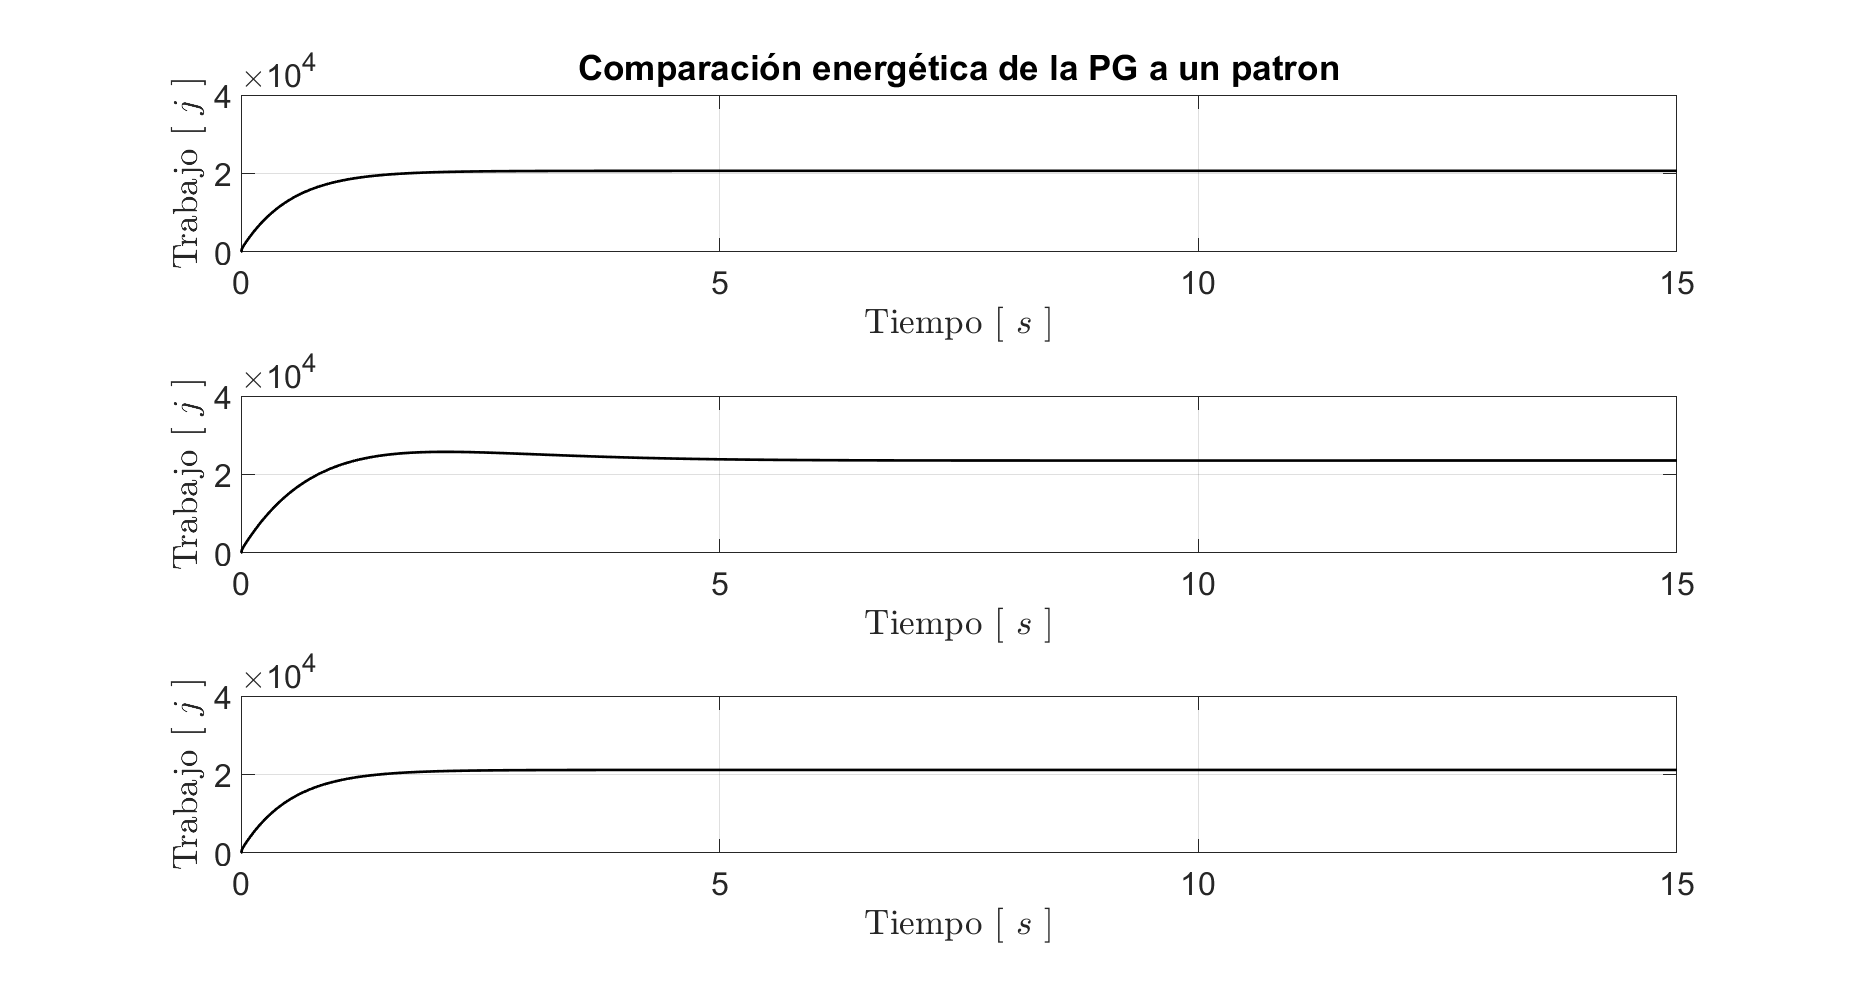
\includegraphics[width=\textwidth]{../03_Reporte/img/energiamovsubplot.png}
 \end{figure}

\end{frame}
